\documentclass{article}

\usepackage{import}
\usepackage{pdfpages}
\usepackage{transparent}
\usepackage{indentfirst}
\usepackage[paper=a4paper, top=2.5cm, bottom=2.5cm, left=2.5cm, right=2.5cm]{geometry} 
\newcommand{\incfig}[2][1]{%
    \def\svgwidth{#1\columnwidth}
    \import{./figures/}{#2.pdf\_tex}
}  

% https://tex.stackexchange.com/questions/141569/highlight-textcolor-and-boldface-simultaneously
\usepackage{xcolor}
\usepackage{color, soul} 
\usepackage{tcolorbox}  % Creating colored boxes  
\counterwithin{table}{section}    

% Add a subsubsubsection 
\newcommand{\subsubsubsection}[1]{\paragraph{#1}\mbox{}}
\setcounter{secnumdepth}{4}
\setcounter{tocdepth}{4}

% Code 
\usepackage{listings}   
\definecolor{dkgreen}{rgb}{0,0.6,0}
\definecolor{gray}{rgb}{0.5,0.5,0.5}
\definecolor{mauve}{rgb}{0.58,0,0.82}

\lstset{frame=tb,
    language=java,
    aboveskip=3mm,
    belowskip=3mm,
    showstringspaces=false,
    columns=flexible,
    basicstyle={\small\ttfamily},
    numbers=none,
    numberstyle=\tiny\color{gray},
    keywordstyle=\color{blue},
    commentstyle=\color{dkgreen},
    stringstyle=\color{mauve},
    breaklines=true,
    breakatwhitespace=true,
    tabsize=3,
}  

\pdfsuppresswarningpagegroup=1 

\title{React JS}
\author{Juliane Marubayashi}
\date{ 2022-07-14 } 


\begin{document}
    \maketitle
    \newpage
    \tableofcontents
    \newpage
    \textbf{Attention before reading}: this document is not original. It is deeply based on the resources.
    Thus, I don't have any credit on the biggest part of this text. 
    \section{React lifecycle}
    React components can go in four different of its life. 

\begin{itemize}
    \item \textbf{Initialization}: In this stage the component is constructed with the given \textbf{props} and default state. 
    This is done in the constructor of the component class. 
    \item \textbf{Mounting}: Is the stage of rendering the JSX returned by the render method itself.
    \item \textbf{Updating}: The stage the application state is updated and the application is repainted. 
    \item \textbf{Unmounting}: Is the final step where the component will be removed from the page. 
\end{itemize}



\begin{figure}[h]
\centering
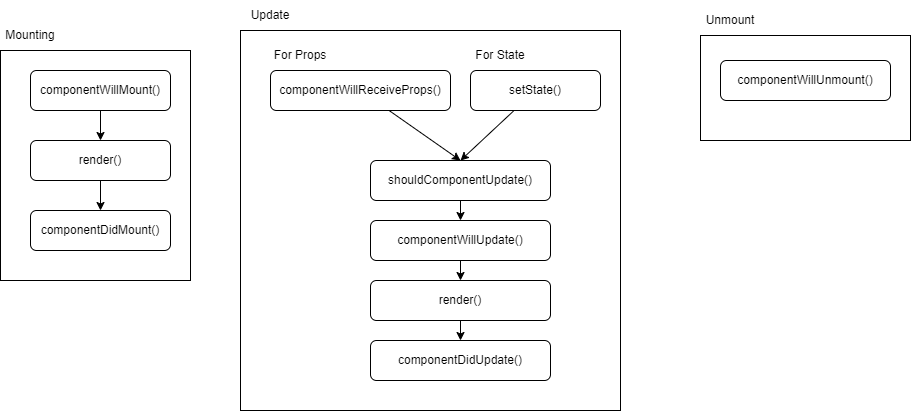
\includegraphics[width=1\linewidth]{figures/01_lifecycle.png}
\caption{React lifecycle}
\label{fig:lifecycle}
\end{figure}

https://www.geeksforgeeks.org/reactjs-lifecycle-components/


    \section{React Use Effect}
    You can think of \texttt{useEffect} as \texttt{componentDidMount}, \texttt{componentDidUpdate},
and \texttt{componentWillUnmount} combined. 

\subsection{Effect without cleanup}

Sometimes, we want to run some additional code \textbf{after} React component
has updated the DOM. 
In React the \texttt{render} method, shouldn't cause any side effect. We usually
want to perform effect \textbf{after} React has updated the DOM. 

This is why usually we put side effects in \texttt{componentDidMount} and 
\texttt{componentDidUpdate}. 

An example is:

\begin{lstlisting}
class Example extends React.Component {
  constructor(props) {
    super(props);
    this.state = {
      count: 0
    };
  }

  componentDidMount() {
    document.title = `You clicked ${this.state.count} times`;
  }
  componentDidUpdate() {
    document.title = `You clicked ${this.state.count} times`;
  }

  render() {
    return (
      <div>
        <p>You clicked {this.state.count} times</p>
        <button onClick={() => this.setState({ count: this.state.count + 1 })}>
          Click me
        </button>
      </div>
    );
  }
}
\end{lstlisting}


\end{document}  

% ---------------------
% Bibliography
% --------------------- 
% A folder bst/report.bib should be created 
\bibliographystyle{unsrt}
\bibliography{bst/report}  


